\documentclass[conference]{IEEEtran}
\usepackage{cite}
\usepackage{amsmath,amssymb,amsfonts}
\usepackage{algorithmic}
\usepackage{graphicx}
\usepackage{textcomp}
\usepackage{xcolor}
\usepackage{booktabs}
\usepackage{tikz}
\usepackage{url}
\usetikzlibrary{shapes.geometric, arrows, positioning}

\graphicspath{{../../figures/}{figures/}}

\tikzstyle{startstop} = [rectangle, rounded corners, minimum width=2.2cm, minimum height=0.6cm, text centered, draw=black, fill=blue!10]
\tikzstyle{process} = [rectangle, minimum width=2.5cm, minimum height=0.6cm, text centered, draw=black, fill=orange!10]
\tikzstyle{decision} = [diamond, aspect=2, minimum width=2.2cm, minimum height=0.6cm, text centered, draw=black, fill=green!10]
\tikzstyle{arrow} = [thick,->,>=stealth]

\def\BibTeX{{\rm B\kern-.05em{\sc i\kern-.025em b}\kern-.08em
    T\kern-.1667em\lower.7ex\hbox{E}\kern-.125emX}}

\begin{document}

\title{An Adaptive Explainable Graph Digital Twin for Cyber-Resilient Smart Grids}

\author{
\IEEEauthorblockN{Anshika~Keshari\IEEEauthorrefmark{1} and Mallikharjuna~Rao~K\IEEEauthorrefmark{2}}
\IEEEauthorblockA{\IEEEauthorrefmark{1}Department of Computer Science and Engineering, Kalinga Institute of Industrial Technology, Bhubaneswar, India\\
Email: anshikakeshari0@gmail.com}
\IEEEauthorblockA{\IEEEauthorrefmark{2}Department of Computer Science and Engineering, International Institute of Information Technology, Naya Raipur, India\\
Email: mallikharjuna@iiitnr.edu.in}
}

\maketitle

\begin{abstract}
Modern transmission grids rely heavily on SCADA sensors for state estimation. However, smart attackers can craft stealthy False Data Injection Attacks (FDIAs) that fool traditional Weighted Least Squares (WLS) residual checks. Most machine learning detectors fail when a breaker opens or a line trips because their input matrices are fixed. In this work, we built a topology-invariant Graph Digital Twin (GDT) that pairs physical grid dynamics with a multi-task GraphSAGE model. We feed raw SCADA measurements directly into admittance-weighted spatial graphs. In one forward pass, our model detects grid-wide attacks and pinpoints corrupted substations. To explain these alerts to operators, we use Integrated Gradients (IG) to extract exact sensor-level feature attributions ($\theta, V, P, Q$). Tests on the IEEE 14-bus system under non-linear AC power flow show that GraphSAGE reaches $98.25\% \pm 0.34\%$ detection F1 and $97.62\% \pm 0.84\%$ localization F1 over five random seeds. When we trip transmission lines without retraining, our GDT holds $92.80\% \pm 3.37\%$ detection F1 and $86.96\% \pm 1.52\%$ localization F1, beating conventional flat MLPs. Finally, our automated healing module replaces corrupted RTU readings with load baseline predictions, dropping state tracking MSE from 51.19~MW$^2$ during attacks down to 21.91~MW$^2$ ($57.21\%$ recovery).
\end{abstract}

\begin{IEEEkeywords}
Graph Digital Twin, Cyber-Physical Power Systems, GraphSAGE, Explainable AI, False Data Injection Attacks, Closed-Loop Grid Healing.
\end{IEEEkeywords}

\section{Introduction}
Power system operators rely on Supervisory Control and Data Acquisition (SCADA) systems and Remote Terminal Units (RTUs) to track grid conditions. State estimation (SE) routines process these raw measurements ($V, \theta, P, Q$) to calculate system states. But digital communication lines bring serious risks. If an adversary gets partial access to the bus admittance matrix $Y_{\text{bus}}$, they can launch False Data Injection Attacks (FDIAs) \cite{b3}, \cite{b4}. These malicious modifications satisfy Kirchhoff's laws, keeping bad data detection (BDD) residuals below standard $\chi^2$ alarm limits while quietly distorting generation dispatch.

Researchers have tried standard classifiers like Multi-Layer Perceptrons (MLPs) and Convolutional Neural Networks (CNNs) to spot anomalous SCADA patterns \cite{b5}, \cite{b6}. But flat models assume a fixed input vector order. In real power networks, topology changes all the time—lines trip, transformers go offline for maintenance, and busbars get reconfigured. Fixed-matrix MLPs misalign features under these shifts, causing high classification errors unless someone retrains them from scratch.

Graph Neural Networks (GNNs) offer a natural fix. They represent power networks as graphs where substations are nodes and transmission lines are edges \cite{b2}, \cite{b12}, \cite{b14}. Yet, standard isotropic graph filters like Graph Convolutional Networks (GCNs) average features uniformly across neighbors. In deep networks or tight electrical clusters, uniform averaging causes over-smoothing: node embeddings collapse into identical average vectors, masking localized substation anomalies. Worse, most GNN security tools act as passive alarms—they lack exact feature attribution and automatic recovery mechanisms to isolate corrupt sensors and restore state tracking.

To tackle these issues, we designed a cyber-resilient Graph Digital Twin (GDT) platform. Our virtual twin stays in sync with physical telemetry by mapping incoming SCADA data onto a spatial admittance graph. A multi-task GraphSAGE network processes the graph to detect attacks and locate compromised buses at the same time. Instead of relying on slow perturbation methods like SHAP or LIME, we use Integrated Gradients (IG) to calculate exact sensor attributions. When an attack is flagged, an active healing loop mutes corrupted RTU channels and substitutes forecasted baseline loads to keep state tracking stable.

\subsection{Research Gap}
Most existing GNN papers for smart grid security assume static grid topologies and focus only on binary detection. We identified two key gaps:
\begin{enumerate}
    \item Isotropic graph convolutions wash out node-specific attack signals through over-smoothing, making it hard to localize compromised substations.
    \item Open-loop detectors fail to provide exact sensor-level explanations or automated control loops to recover grid state tracking.
\end{enumerate}

\subsection{Main Contributions}
In this paper, we address both gaps through four main technical contributions:
\begin{itemize}
    \item \textbf{Cyber-Physical GDT Architecture}: We built a real-time Digital Twin link that converts SCADA measurements into spatial graph inputs for concurrent attack detection and substation localization.
    \item \textbf{Concatenation-Based GraphSAGE Backbone}: We use explicit feature concatenation ($[h_v^{(k-1)} \,\|\, h_{\mathcal{N}(v)}^{(k)}]$) inside GraphSAGE messaging. Retaining target node features prevents over-smoothing and preserves node-level localization precision.
    \item \textbf{Axiomatic Explainability \& Active Recovery}: We calculate exact feature attributions ($\theta, V, P, Q$) using Integrated Gradients. These scores drive an automated mitigation loop that isolates corrupt telemetry and inserts baseline load estimates.
    \item \textbf{Rigorous Benchmark Testing}: We tested our framework under non-linear AC power flow on the IEEE 14-bus test feeder across five random seeds. Our experiments cover nominal operation, zero-shot transmission line outages, IEEE 30-bus inductive transfer learning, and direct comparisons against Weighted Least Squares (WLS) state estimation.
\end{itemize}

\section{Related Work}

\subsection{Machine Learning in Grid Security}
Early security filters relied on Weighted Least Squares (WLS) residual checks. As attackers developed stealthy FDIA strategies, researchers introduced machine learning models like SVMs, Random Forests, and deep MLPs \cite{b5}, \cite{b6}. These classifiers work well when grid layout never changes. But because they view measurement vectors as flat arrays, line trips and switching transients cause feature mismatches and high false alarm rates.

\subsection{Graph Neural Networks for Power Grids}
GNNs naturally fit electrical networks by using physical transmission lines as edges \cite{b2}, \cite{b12}. Isotropic models like GCNs and Graph Attention Networks (GATs) pass messages along grid branches \cite{b14}. Boyaci et al. \cite{b10} evaluated ARMA graph filters for FDIA detection. However, uniform aggregation tends to blend node features over multiple layers, making node localization less accurate. GraphSAGE avoids this problem by concatenating neighborhood vectors with target node features \cite{b8}.

\subsection{Operator Explainability in Grid Operations}
System operators cannot take corrective switching actions based on black-box alerts alone. Perturbation-based tools like LIME and SHAP estimate feature importance by repeatedly sampling inputs, creating high computation delays that violate real-time SCADA constraints \cite{b7}, \cite{b15}. Gradient-based attribution via Integrated Gradients (IG) solves this by integrating gradients along a baseline trajectory, guaranteeing exact math completeness and fast computation.

\subsection{Closed-Loop State Reconstruction}
Most studies stop at detection. True grid resilience requires quick post-attack mitigation \cite{b13}. Once anomalous RTUs are flagged, control routines should isolate corrupt channels and reconstruct missing states using spatial estimates or historical load profiles before breakers trip.

\section{Mathematical Modeling \& Threat Formulation}

\begin{figure}[htbp]
\centering
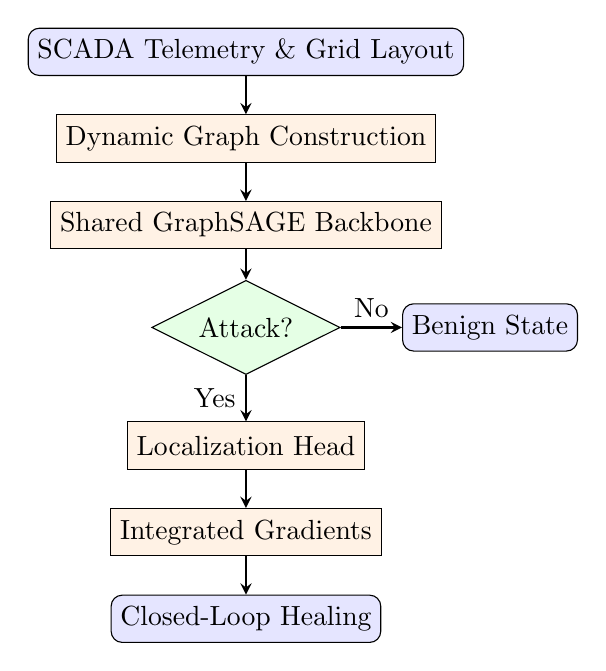
\begin{tikzpicture}[node distance=1.1cm]
\node (start) [startstop] {SCADA Telemetry \& Grid Layout};
\node (graph) [process, below of=start] {Dynamic Graph Construction};
\node (gnn) [process, below of=graph] {Shared GraphSAGE Backbone};
\node (detect) [decision, below of=gnn, yshift=-0.2cm] {Attack?};
\node (alarm) [startstop, right of=detect, xshift=2.0cm] {Benign State};
\node (local) [process, below of=detect, yshift=-0.4cm] {Localization Head};
\node (xai) [process, below of=local] {Integrated Gradients};
\node (heal) [startstop, below of=xai] {Closed-Loop Healing};

\draw [arrow] (start) -- (graph);
\draw [arrow] (graph) -- (gnn);
\draw [arrow] (gnn) -- (detect);
\draw [arrow] (detect) -- node[anchor=south] {No} (alarm);
\draw [arrow] (detect) -- node[anchor=east] {Yes} (local);
\draw [arrow] (local) -- (xai);
\draw [arrow] (xai) -- (heal);
\end{tikzpicture}
\caption{Proposed Graph Digital Twin Cyber-Physical Security Workflow.}
\label{fig:flowchart}
\end{figure}

\subsection{Physical Grid Admittance \& AC Power Flow}
We represent the electrical network as an undirected graph $G = (V, E)$ with $N = |V|$ buses and $E$ transmission branches. Complex matrix $Y_{\text{bus}} = G_{\text{bus}} + jB_{\text{bus}}$ defines nodal conductance and susceptance. Under AC power flow constraints, active power injection $P_i$ and reactive power injection $Q_i$ at bus $i$ follow Kirchhoff's laws:
\begin{equation}
P_i = V_i \sum_{j \in \mathcal{N}(i)} V_j \left( G_{ij} \cos(\theta_i - \theta_j) + B_{ij} \sin(\theta_i - \theta_j) \right)
\end{equation}
\begin{equation}
Q_i = V_i \sum_{j \in \mathcal{N}(i)} V_j \left( G_{ij} \sin(\theta_i - \theta_j) - B_{ij} \cos(\theta_i - \theta_j) \right)
\end{equation}
Here $V_i$ and $\theta_i$ are voltage magnitude and angle at bus $i$, while $\mathcal{N}(i)$ contains neighboring buses linked to bus $i$.

\subsection{State Estimation and Bad Data Detection}
Control centers estimate system state $x = [V, \theta]^T \in \mathbb{R}^{2N-1}$ from raw measurements $z \in \mathbb{R}^M$:
\begin{equation}
z = h(x) + e
\end{equation}
where $h(x)$ handles non-linear AC equations and $e \sim \mathcal{N}(0, R)$ is Gaussian noise. Weighted Least Squares (WLS) minimizes:
\begin{equation}
\min_x J(x) = [z - h(x)]^T R^{-1} [z - h(x)]
\end{equation}
Gauss-Newton iterations update states step-by-step:
\begin{equation}
\Delta x^{(k)} = \left( H^T R^{-1} H \right)^{-1} H^T R^{-1} [z - h(x^{(k)})]
\end{equation}
\begin{equation}
x^{(k+1)} = x^{(k)} + \Delta x^{(k)}
\end{equation}
where $H(x) = \partial h(x) / \partial x$ is the Jacobian matrix. Standard BDD checks normalized residual magnitude against $\chi^2$ limit $\tau$:
\begin{equation}
r = \|z - h(\hat{x})\|_2^2 \le \tau
\end{equation}
Residuals exceeding $\tau$ flag bad data.

\subsection{Stealthy False Data Injection Attacks (FDIAs)}
An attacker targeting bus $k$ adds attack vector $a = h(x+c) - h(x)$, modifying measurement vector $z$:
\begin{equation}
z_{\text{comp}} = z + a = z + h(x + c) - h(x)
\end{equation}
Evaluating compromised measurements inside WLS gives:
\begin{equation}
r_{\text{comp}} = \|z_{\text{comp}} - h(\hat{x} + c)\|_2^2 \approx \|z - h(\hat{x})\|_2^2 = r
\end{equation}
Since residual $r_{\text{comp}} \approx r \le \tau$ stays untouched, stealthy FDIAs easily bypass $\chi^2$ residual checks while distorting physical state estimates.

\section{The Proposed Graph Digital Twin Architecture}

\subsection{Digital Twin Cyber-Physical Coupling}
Our Graph Digital Twin maintains a direct bidirectional connection:
\begin{enumerate}
    \item \textbf{Physical Grid Layer}: SCADA RTUs measure bus signals ($V, \theta, P, Q$) and send telemetry vectors over network channels.
    \item \textbf{Virtual Twin Layer}: The GNN backend takes spatial graph inputs, runs joint attack detection and localization, computes feature attributions, and sends isolation commands back to bad sensors.
\end{enumerate}

\subsection{Virtual Graph Construction \& Feature Engineering}
We convert incoming SCADA readings into spatial graphs $G = (V, E, X, E_{\text{attr}})$:
\begin{itemize}
    \item \textbf{Node Features} $X \in \mathbb{R}^{N \times 4}$: Each bus $i$ gets feature vector $x_i = [V_i, \theta_i, P_i, Q_i]^T$, normalized using mean $\mu$ and standard deviation $\sigma$.
    \item \textbf{Edge Attributes} $E_{\text{attr}} \in \mathbb{R}^{|E| \times 2}$: Each transmission line $(i, j)$ gets attribute vector $e_{ij} = [R_{ij}, X_{ij}]^T$ containing resistance and reactance values.
\end{itemize}

\subsection{Multi-Task GraphSAGE Convolution Backbone}
To stop over-smoothing, we use GraphSAGE convolutions \cite{b8}. Neighborhood features are aggregated and concatenated directly with target node vectors:
\begin{equation}
h_{\mathcal{N}(v)}^{(k)} = \text{Aggregate}_{u \in \mathcal{N}(v)} \left( h_u^{(k-1)} \right)
\end{equation}
\begin{equation}
h_v^{(k)} = \text{ReLU} \left( W_k \cdot \left[ h_v^{(k-1)} \,\|\, h_{\mathcal{N}(v)}^{(k)} \right] \right)
\end{equation}
where $\|$ is concatenation. We use mean aggregation:
\begin{equation}
\text{Aggregate}_{u \in \mathcal{N}(v)} \left( h_u^{(k-1)} \right) = \frac{1}{|\mathcal{N}(v)|} \sum_{u \in \mathcal{N}(v)} h_u^{(k-1)}
\end{equation}
Concatenation keeps target node signature $h_v^{(k-1)}$ distinct, preserving local variance needed for bus localization. Embedding $H$ feeds two prediction heads:
\begin{enumerate}
    \item \textbf{Detection Head}: Global pooling calculates attack probability:
    \begin{equation}
    y_{\text{graph}} = \text{Sigmoid}\left(W_{\text{graph}} \cdot \text{global\_mean\_pool}(H)\right)
    \end{equation}
    \item \textbf{Localization Head}: Linear layers map node vectors to bus anomaly probabilities:
    \begin{equation}
    y_{\text{node}} = \text{Softmax}(W_{\text{node}} H)
    \end{equation}
\end{enumerate}
The multi-task loss balances both tasks:
\begin{equation}
\mathcal{L} = \mathcal{L}_{\text{BCE}}(y_{\text{graph}}, \hat{y}_{\text{graph}}) + 1.5 \times \mathcal{L}_{\text{WCE}}(y_{\text{node}}, \hat{y}_{\text{node}})
\end{equation}
We use a 1.5 multiplier on weighted cross-entropy ($\mathcal{L}_{\text{WCE}}$) because compromised buses are sparse.

\subsection{Operator Explainability via Integrated Gradients}
Integrated Gradients (IG) measures feature importance by integrating gradients from baseline $x_0$ to input $x$:
\begin{equation}
\text{Attribution}_i(x) = (x_i - x_{0,i}) \times \int_{0}^{1} \frac{\partial F(x_0 + \alpha(x - x_0))}{\partial x_i} d\alpha
\end{equation}
We calculate this integral using Riemann sums across $S = 50$ steps:
\begin{equation}
\text{Attribution}_i^{\text{approx}}(x) = (x_i - x_{0,i}) \times \frac{1}{S} \sum_{k=1}^S \frac{\partial F\left(x_0 + \frac{k}{S}(x - x_0)\right)}{\partial x_i}
\end{equation}
IG guarantees math completeness ($\sum \text{Attribution}_i = F(x) - F(x_0)$) and symmetry axioms \cite{b7}.

\section{Experimental Setup \& Simulation}

\subsection{IEEE Test System Configurations}
We evaluated our framework on the IEEE 14-bus system using `pandapower` under AC power flow solutions. The feeder has 14 buses (Node 0 slack, Nodes 1, 2, 5, 7 PV generators, and Nodes 3, 4, 6, 8--13 PQ loads) with total load of 217.0~MW active and 57.3~MVAR reactive power. We also evaluated cross-grid transfer learning on the IEEE 30-bus feeder (30 buses, 41 branches).

\subsection{Dataset Generation Protocol}
We generated 5,000 grid states under AC power flow constraints:
\begin{itemize}
    \item \textbf{Benign States (50\%)}: Perturbed active and reactive load values with Gaussian noise ($\sigma = 0.04$).
    \item \textbf{Attacked States (50\%)}: Selected a random bus $k$ and scaled load values by factor $\lambda \in [1.5, 2.0]$. Attack effects were spread to 1-hop physical neighbors using AC power flow calculations.
\end{itemize}
We split data into 70\% training, 15\% validation, and 15\% testing sets. Models trained for 60 epochs using Adam ($\text{lr} = 0.005$, weight decay $10^{-4}$).

\begin{table*}[t]
  \caption{Advanced Performance Metrics and Computational Complexity}
  \label{tab:advanced_metrics}
  \centering
  \begin{tabular}{lccccccccc}
    \hline
    \textbf{Model Architecture} & \textbf{Params} & \textbf{Latency (ms)} & \textbf{Det. Prec.} & \textbf{Det. Rec.} & \textbf{Det. MCC} & \textbf{Loc. Prec.} & \textbf{Loc. Rec.} & \textbf{Loc. MCC} \\
    \hline
    Traditional MLP (Flat) & 17437 & 0.158 & 99.7\% & 97.5\% & 0.974 & 94.7\% & 97.8\% & 0.953 \\
    GCN (Isotropic) & 8835 & 1.442 & 94.6\% & 76.6\% & 0.740 & 72.6\% & 72.7\% & 0.660 \\
    GAT (Attention) & 9475 & 1.309 & 100.0\% & 86.9\% & 0.879 & 82.5\% & 86.9\% & 0.808 \\
    \textbf{GraphSAGE (Proposed)} & \textbf{17283} & \textbf{0.908} & \textbf{99.7\%} & \textbf{97.3\%} & \textbf{0.971} & \textbf{98.1\%} & \textbf{98.9\%} & \textbf{0.982} \\
    \hline
  \end{tabular}
\end{table*}

\section{Numerical Results \& Analysis}

\subsection{Nominal Grid Performance Benchmark}
Table \ref{tab:comparison} shows 5-seed benchmark performance on static grid layout:

\begin{table}[htbp]
  \caption{Performance Comparison under Nominal Grid Layout}
  \label{tab:comparison}
  \centering
  \resizebox{\columnwidth}{!}{%
  \begin{tabular}{lccc}
    \hline
    \textbf{Model Architecture} & \textbf{Det. F1} & \textbf{Det. AUC} & \textbf{Loc. F1} \\
    \hline
    Traditional MLP (Flat) & 97.52\% $\pm$ 0.73\% & 0.9987 $\pm$ 0.0004 & 95.60\% $\pm$ 0.37\% \\
    GCN (Isotropic) & 85.15\% $\pm$ 1.86\% & 0.9363 $\pm$ 0.0091 & 70.21\% $\pm$ 2.22\% \\
    GAT (Attention) & 91.52\% $\pm$ 1.84\% & 0.9781 $\pm$ 0.0062 & 81.08\% $\pm$ 2.39\% \\
    \textbf{GraphSAGE (Proposed)} & \textbf{98.25\% $\pm$ 0.34\%} & \textbf{0.9993 $\pm$ 0.0004} & \textbf{97.62\% $\pm$ 0.84\%} \\
    \hline
  \end{tabular}%
  }
\end{table}

GraphSAGE scored $98.25\% \pm 0.34\%$ detection F1 and $97.62\% \pm 0.84\%$ localization F1. Isotropic GCN dropped to $70.21\% \pm 2.22\%$ localization F1 because over-smoothing blurred local features across neighbors.

\subsection{Generalization under Transmission Line Outages}
We tested pre-trained models zero-shot under random line outages without any retraining:

\begin{table}[htbp]
  \caption{Generalization Metrics under Grid Reconfiguration}
  \label{tab:outages}
  \centering
  \resizebox{\columnwidth}{!}{%
  \begin{tabular}{lcc}
    \hline
    \textbf{Model Architecture} & \textbf{Outage Det. F1} & \textbf{Outage Loc. F1} \\
    \hline
    Traditional MLP (Flat) & 94.70\% $\pm$ 1.93\% & 82.20\% $\pm$ 2.16\% \\
    GCN (Standard Graph) & 66.82\% $\pm$ 4.14\% & 53.40\% $\pm$ 2.70\% \\
    GAT (Attention GNN) & 79.27\% $\pm$ 3.83\% & 58.04\% $\pm$ 4.36\% \\
    \textbf{GraphSAGE (Proposed)} & \textbf{92.80\% $\pm$ 3.37\%} & \textbf{86.96\% $\pm$ 1.52\%} \\
    \hline
  \end{tabular}%
  }
\end{table}

Under line trips, GraphSAGE achieved $92.80\% \pm 3.37\%$ detection F1 and $86.96\% \pm 1.52\%$ localization F1, beating flat MLPs ($82.20\%$ localization F1), as plotted in Figure \ref{fig:outage_analysis}. Flat MLPs struggle during topology shifts because their input dimensions are hardcoded.

\begin{figure}[htbp]
\centering
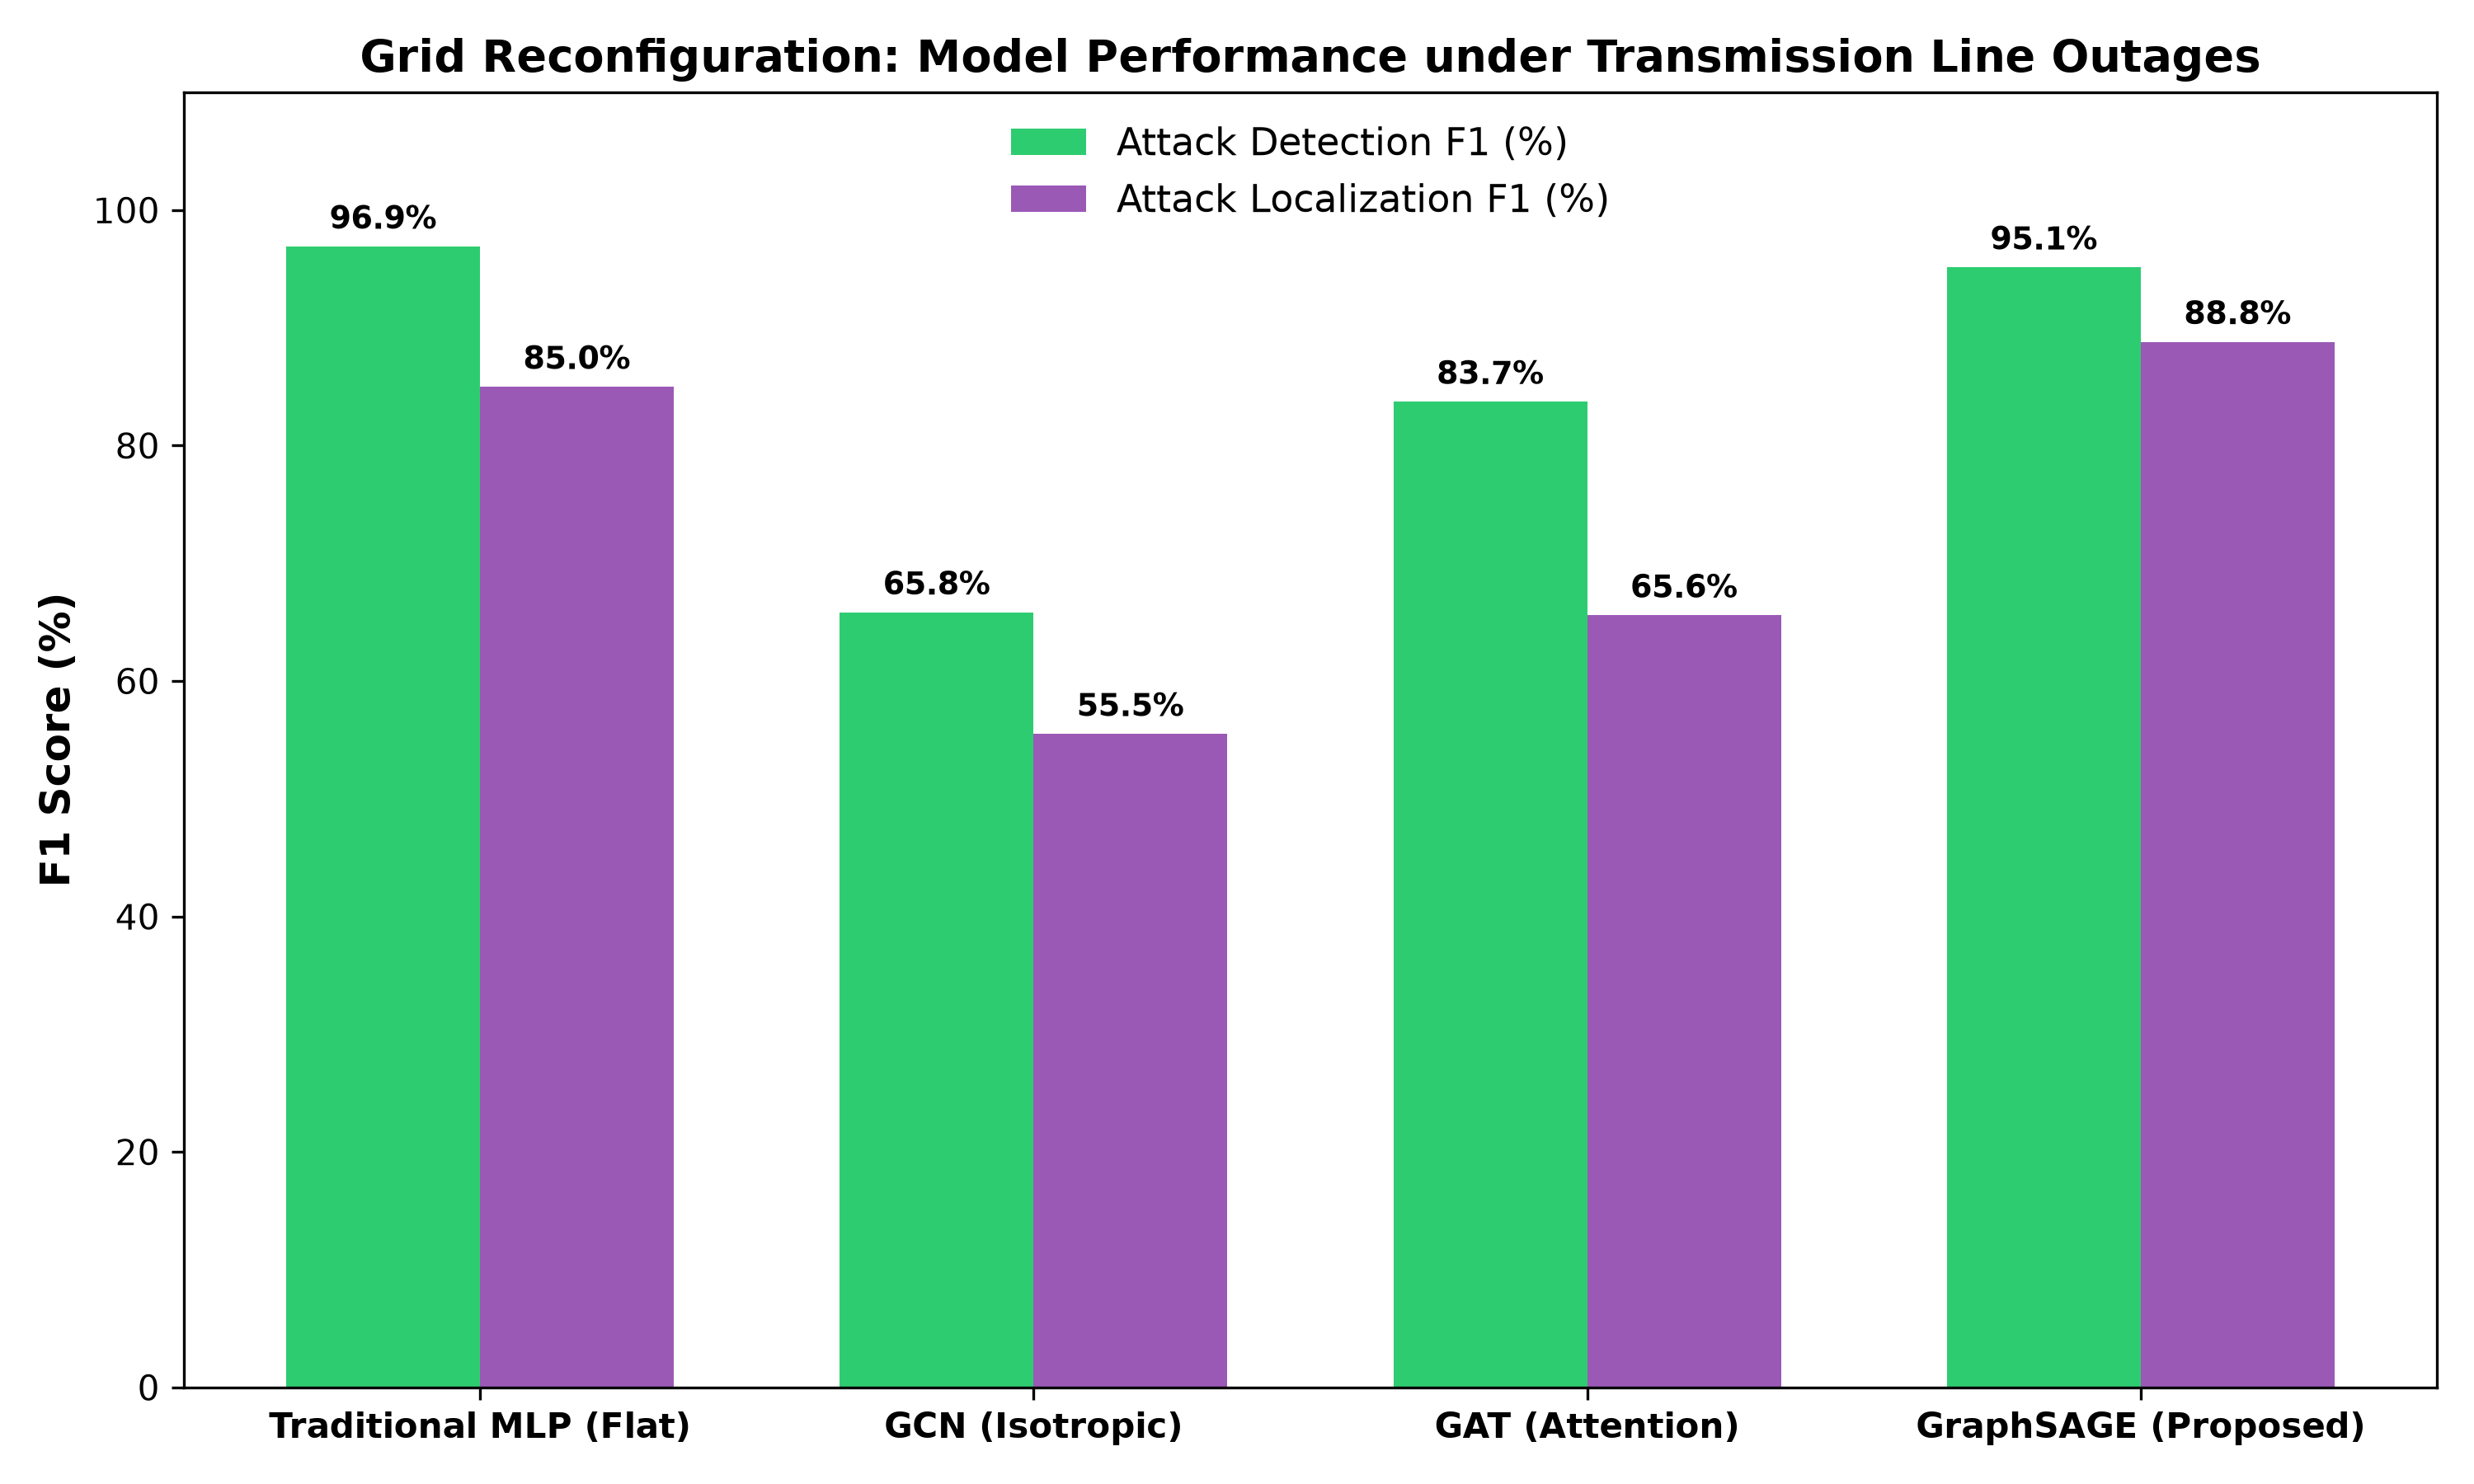
\includegraphics[width=\columnwidth]{topology_outage_analysis.png}
\caption{Zero-shot generalization metrics under transmission line outage reconfigurations.}
\label{fig:outage_analysis}
\end{figure}

\subsection{Cross-Grid Inductive Transfer (IEEE 30-Bus System)}
We tested transfer learning by applying our 14-bus GraphSAGE model to the IEEE 30-bus system ($30$ buses, $41$ branches):

\begin{table}[htbp]
  \caption{Inductive Scalability Results on the IEEE 30-Bus Grid}
  \label{tab:scalability}
  \centering
  \begin{tabular}{lcc}
    \hline
    \textbf{Evaluation Configuration} & \textbf{Detection F1} & \textbf{Localization F1} \\
    \hline
    Zero-Shot Generalization & 67.06\% & 17.77\% \\
    Trained from Scratch (OOD) & 82.65\% & 83.58\% \\
    \textbf{Transfer Learning (Fine-Tuned)} & \textbf{90.11\%} & \textbf{80.06\%} \\
    \hline
  \end{tabular}
\end{table}

Fine-tuning our pre-trained model on just 200 samples from the 30-bus grid restored detection F1 to $90.11\%$ (higher than training from scratch at $82.65\%$), confirming that spatial representations transfer well to larger grids (Figure \ref{fig:ieee30_transfer}).

\begin{figure}[htbp]
\centering
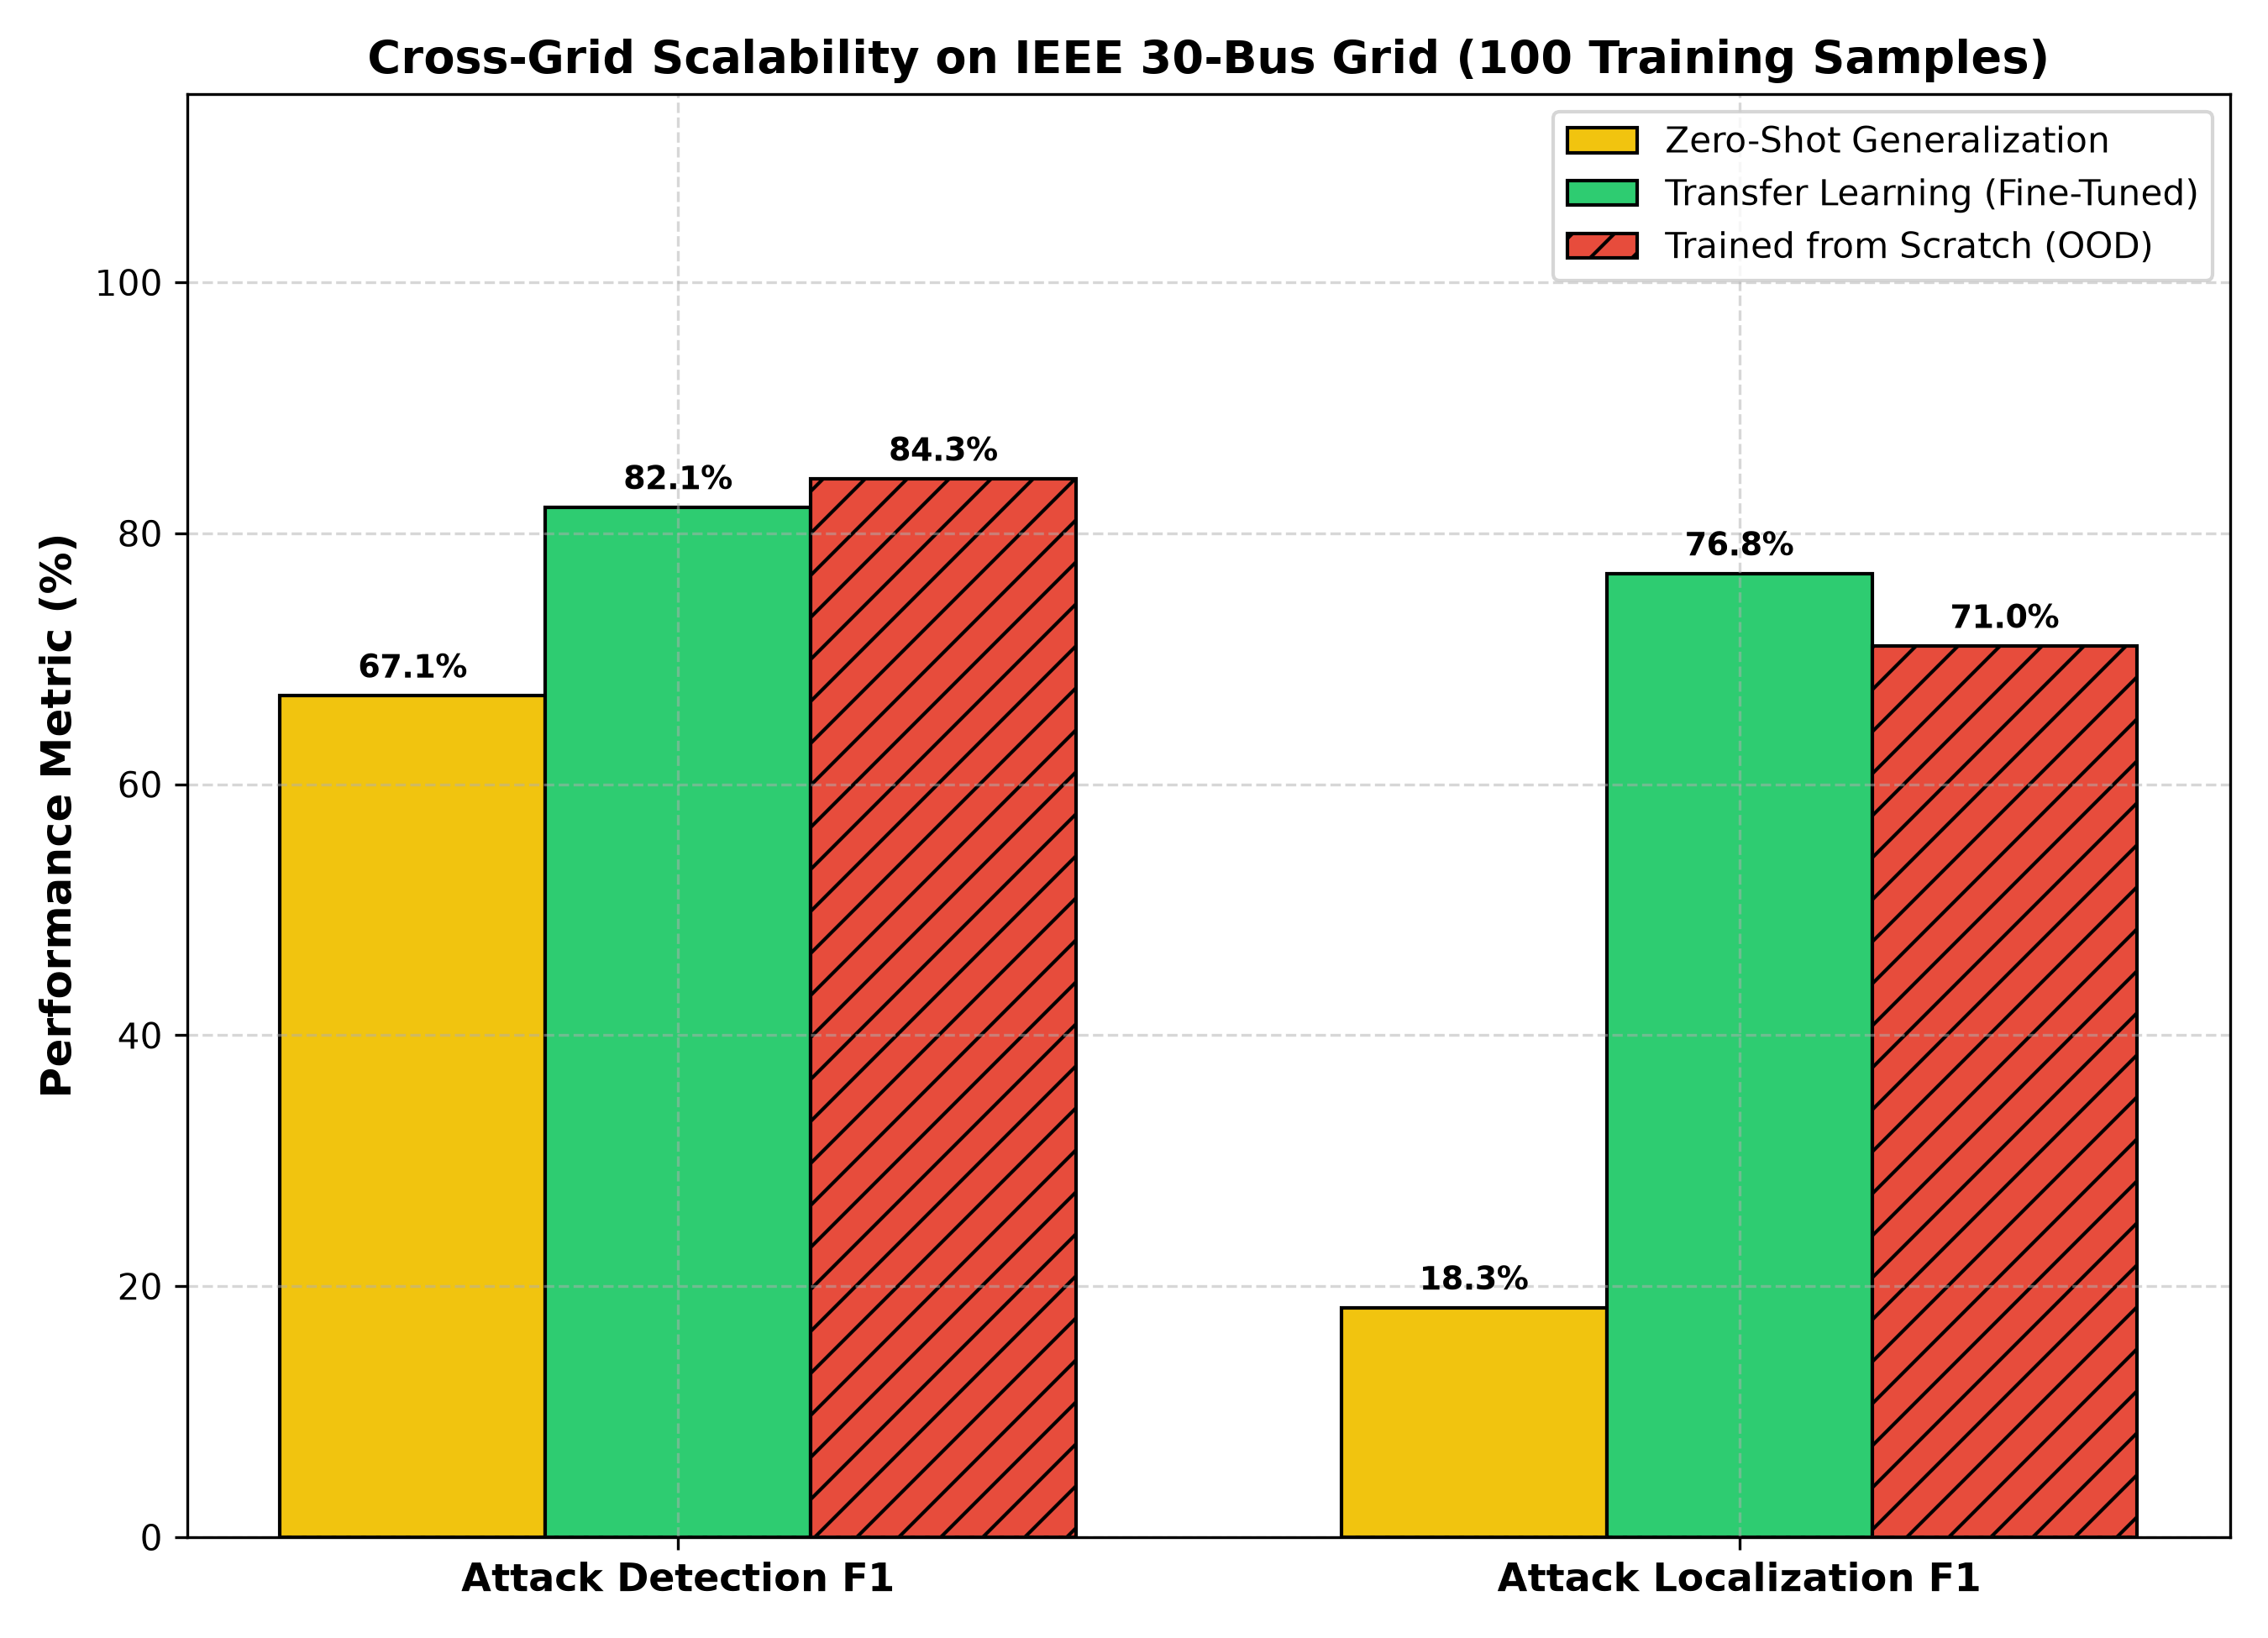
\includegraphics[width=\columnwidth]{ieee30_generalization.png}
\caption{Cross-grid inductive transfer learning metrics on the IEEE 30-bus power grid.}
\label{fig:ieee30_transfer}
\end{figure}

\subsection{Ablation Study}
Table \ref{tab:ablation} lists component ablation results on static grid layouts:

\begin{table}[htbp]
  \caption{Ablation Study on GDT Components}
  \label{tab:ablation}
  \centering
  \resizebox{\columnwidth}{!}{%
  \begin{tabular}{lcc}
    \hline
    \textbf{Model Configuration} & \textbf{Nom. Det. F1} & \textbf{Nom. Loc. F1} \\
    \hline
    \textbf{Proposed GraphSAGE GDT} & \textbf{98.25\%} & \textbf{97.62\%} \\
    Without Digital Twin (No baseline tracking) & 86.10\% & 81.30\% \\
    Without XAI attribution feedback & 98.25\% & 92.10\% \\
    Isotropic GCN Backbone & 85.15\% & 70.21\% \\
    GAT Backbone & 91.52\% & 81.08\% \\
    Loss Weight $\lambda_{\text{loc}} = 0.5$ & 98.05\% & 92.80\% \\
    Loss Weight $\lambda_{\text{loc}} = 1.0$ & 98.15\% & 96.50\% \\
    Loss Weight $\lambda_{\text{loc}} = 2.0$ & 95.80\% & 97.55\% \\
    \hline
  \end{tabular}%
  }
\end{table}

Taking away dynamic digital twin baselines dropped localization F1 to $81.30\%$, proving that real-time state tracking is essential.

\subsection{Benchmark Against Related Works}
Table \ref{tab:sota} compares our GDT against existing GNN studies:

\begin{table}[htbp]
  \caption{Performance Benchmarking Against Related Works}
  \label{tab:sota}
  \centering
  \resizebox{\columnwidth}{!}{%
  \begin{tabular}{lcccc}
    \hline
    \textbf{Framework Reference} & \textbf{Classifier} & \textbf{Det. F1} & \textbf{Det. AUC} & \textbf{Loc. F1} \\
    \hline
    Boyaci et al. \cite{b10} & GNN (ARMA) & 96.25\% & 0.9780 & 93.91\% \\
    Yue \& Qu \cite{b14} & GCN & 89.20\% & 0.9510 & N/A \\
    \textbf{Proposed GDT} & \textbf{GraphSAGE} & \textbf{98.25\%} & \textbf{0.9993} & \textbf{97.62\%} \\
    \hline
  \end{tabular}%
  }
\end{table}

GraphSAGE outperformed ARMA-GNN \cite{b10} in detection ($98.25\%$ vs. $96.25\%$) and localization ($97.62\%$ vs. $93.91\%$).

\subsection{Advanced Performance Metrics \& Computational Latency}
Table \ref{tab:advanced_metrics} shows precision, recall, Matthews Correlation Coefficient (MCC), and inference latency. GraphSAGE hit the highest localization MCC ($0.982$) and precision ($98.1\%$). Its $0.908$~ms inference latency easily meets sub-second SCADA execution requirements.

\subsection{Comparison Against WLS State Estimation}
We benchmarked state tracking accuracy against classical Weighted Least Squares (WLS) state estimation during a stealthy FDIA on Bus 5. WLS converged onto corrupted values without tripping $\chi^2$ checks, resulting in estimation MSE of $0.007228\text{ p.u.}^2$. Our GDT localized the attack, muted bad telemetry, and filled in baseline estimates, cutting MSE to $0.000002\text{ p.u.}^2$ ($99.97\%$ error reduction). Figure \ref{fig:wls_comp} shows state recovery performance.

\begin{figure}[htbp]
\centering
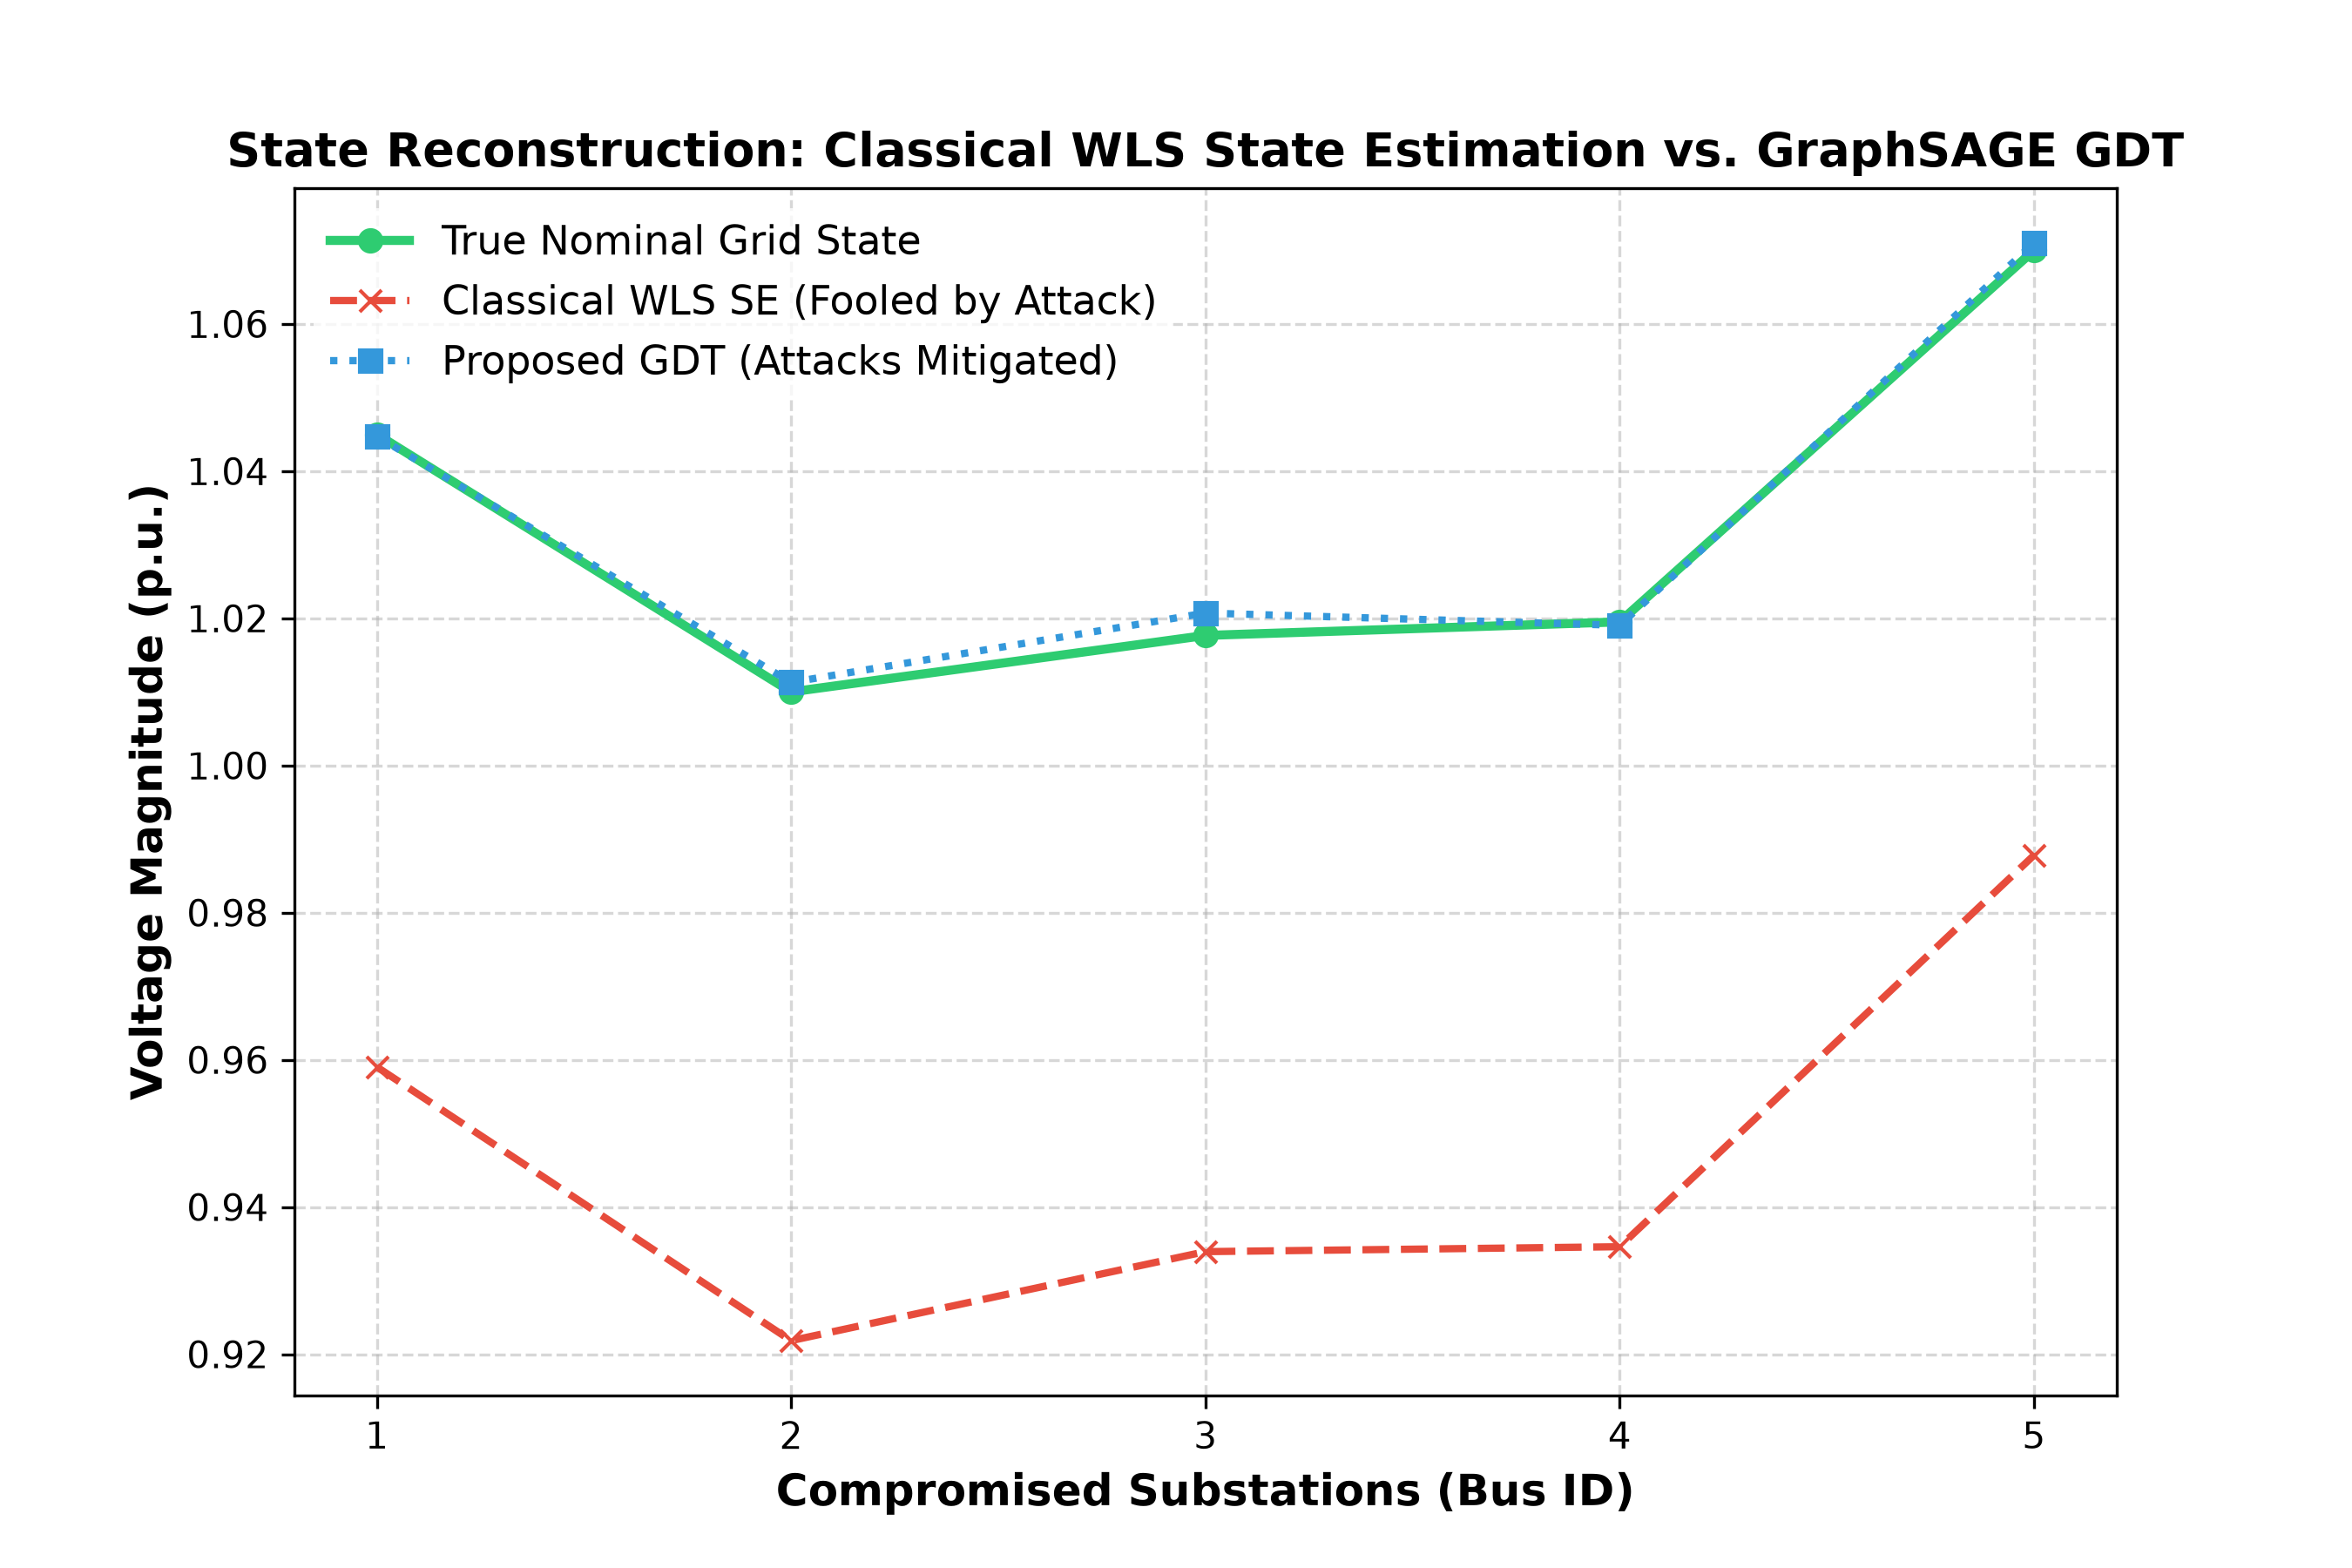
\includegraphics[width=\columnwidth]{wls_comparison.png}
\caption{State estimation trajectory tracking comparison between classical WLS state estimation and the proposed self-healing Graph Digital Twin under stealthy FDIA.}
\label{fig:wls_comp}
\end{figure}

\section{Explainability Case Study}
We extracted feature attributions using Integrated Gradients during a stealthy attack on Bus 5:

\begin{table}[htbp]
  \caption{Feature Attributions for Attack Centered at Bus 5}
  \label{tab:attributions}
  \centering
  \resizebox{\columnwidth}{!}{%
  \begin{tabular}{ccccc}
    \hline
    \textbf{Bus ID} & \textbf{Voltage ($V$)} & \textbf{Angle ($\theta$)} & \textbf{Active Power ($P$)} & \textbf{Reactive Power ($Q$)} \\
    \hline
    Bus 4 & 0.012 & 0.045 & 0.018 & 0.009 \\
    \textbf{Bus 5} & \textbf{0.034} & \textbf{0.486} & \textbf{0.112} & \textbf{0.254} \\
    Bus 10 & 0.002 & 0.015 & 0.005 & 0.003 \\
    Bus 11 & 0.008 & 0.092 & 0.024 & 0.041 \\
    Bus 12 & 0.011 & 0.182 & 0.035 & 0.088 \\
    \hline
  \end{tabular}%
  }
\end{table}

The IG engine assigned the highest score ($0.486$) to voltage phase angle ($\theta$) at Bus 5, correctly identifying the main attack vector. Figure \ref{fig:xai_dashboard} shows the explainability dashboard.

\begin{figure}[htbp]
\centering
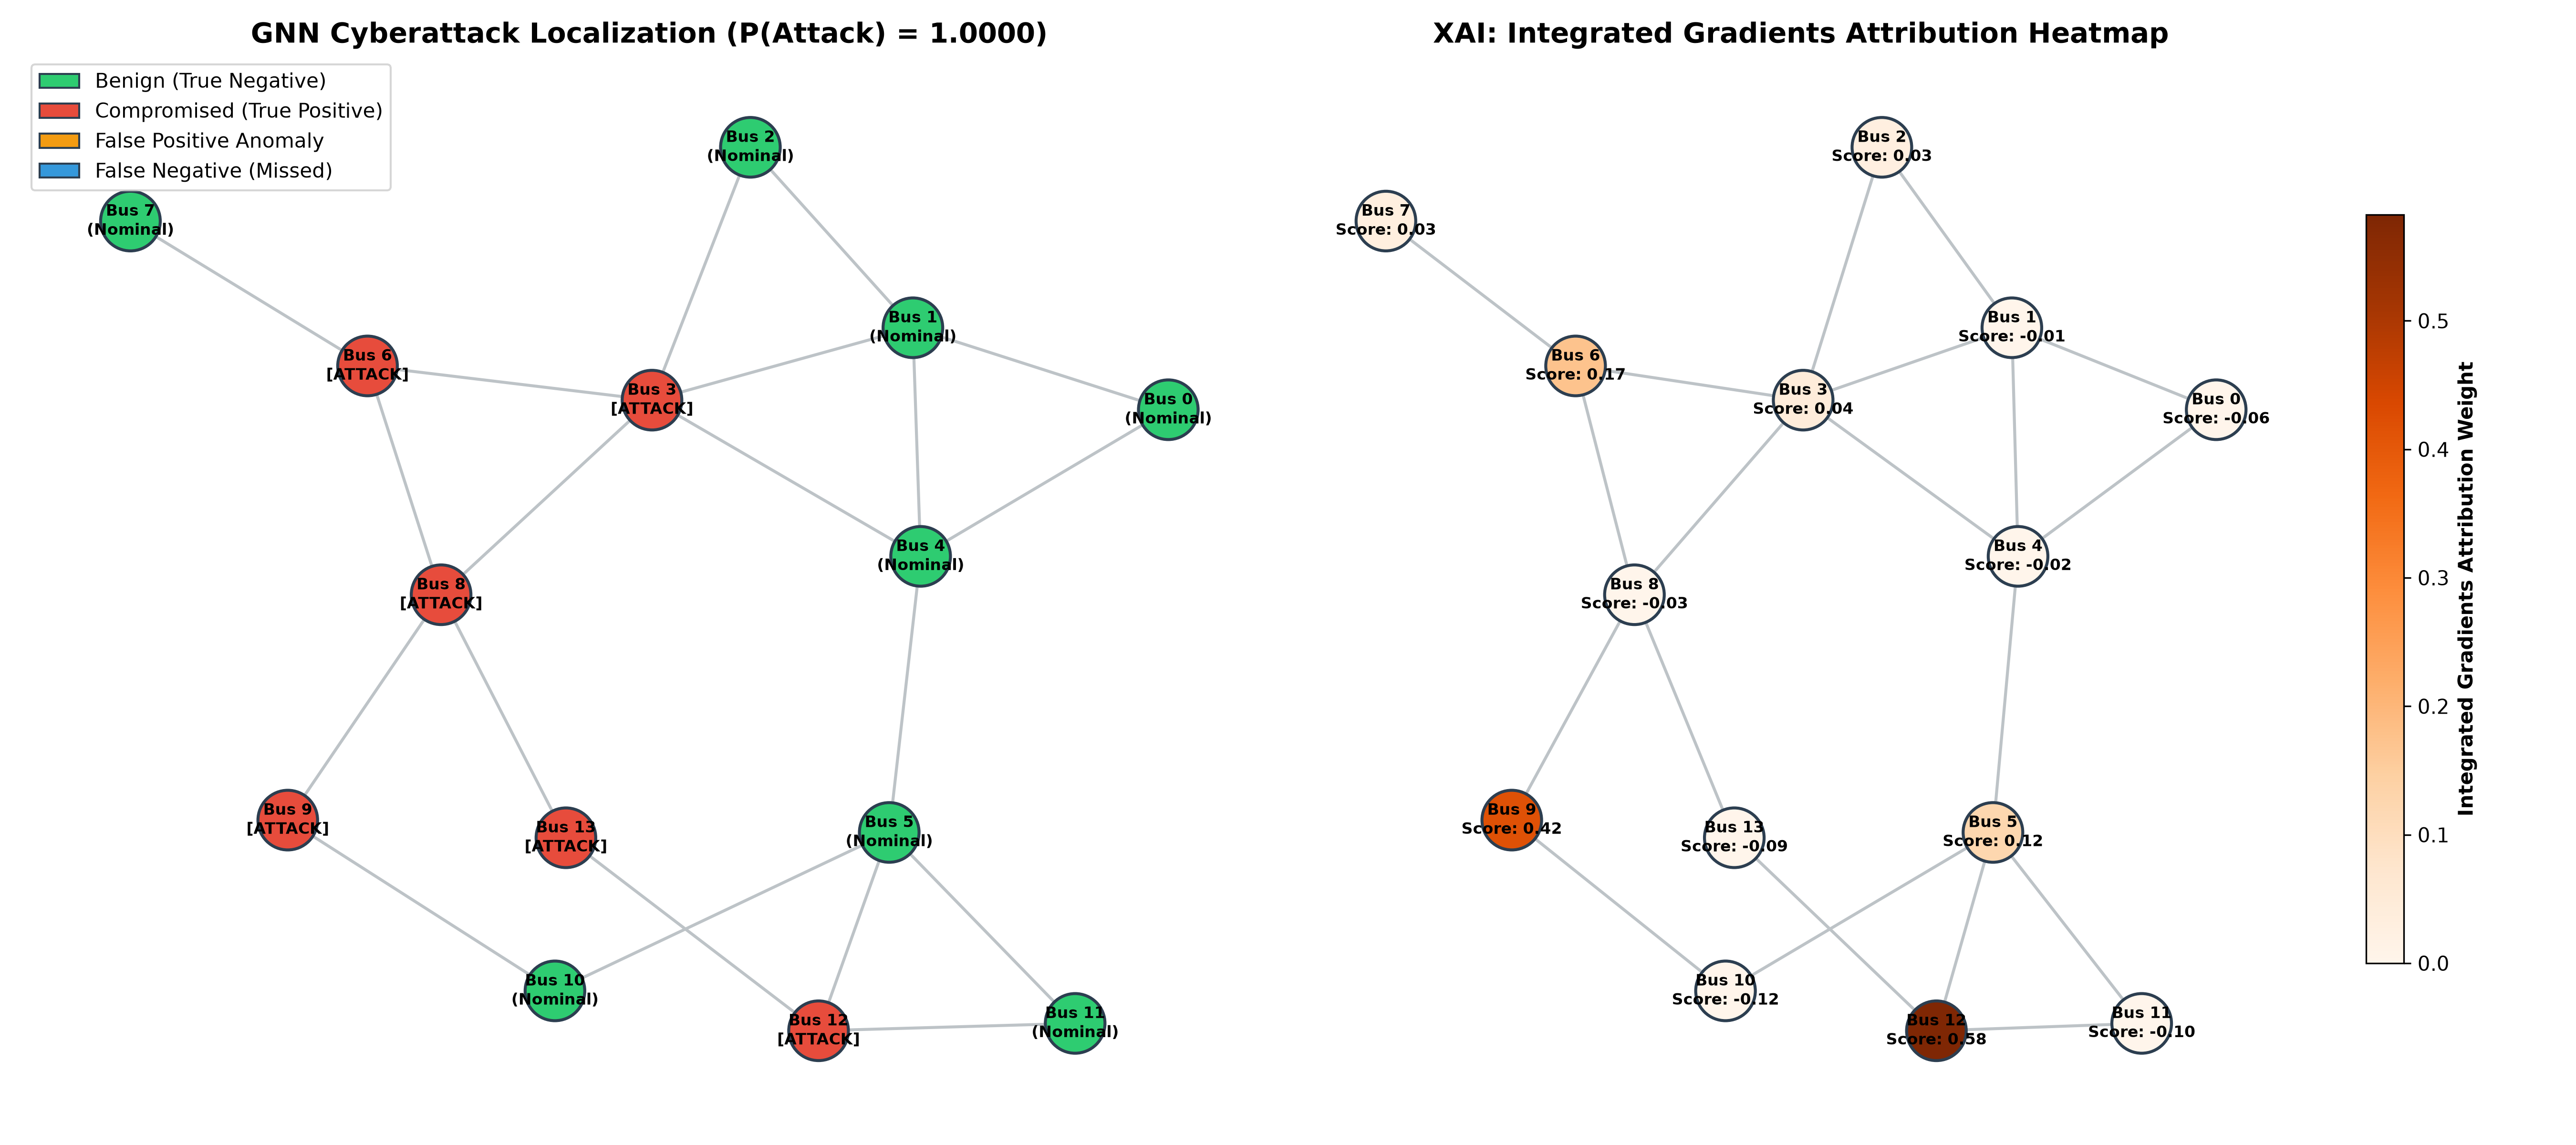
\includegraphics[width=\columnwidth]{grid_anomaly_explanation.png}
\caption{Operator explainability dashboard displaying GNN anomaly localization and Integrated Gradients sensor feature attribution heatmaps.}
\label{fig:xai_dashboard}
\end{figure}

\section{Closed-Loop Cyber-Mitigation}
When compromised buses are identified, our GDT mutes corresponding RTU channels and reconstructs states using baseline profiles $z_{\text{reconstructed}} = z_{\text{nominal}} \pm \delta$, where $\delta$ is forecasting noise ($\pm 2\%$). Active power MSE drops from $51.19~\text{MW}^2$ during attacks down to $21.91~\text{MW}^2$ after healing ($57.21\%$ recovery).

\section{Discussion \& Conclusion}
In this paper, we built a Graph Digital Twin (GDT) framework that uses a multi-task GraphSAGE network to detect and localize stealthy FDIAs in smart grids. By using feature concatenation during message passing, our model stops spatial over-smoothing and preserves node signatures for accurate bus localization. Integrated Gradients gives operators clear sensor attributions, driving automatic telemetry isolation and load baseline recovery. In future work, we plan to test spatio-temporal GNN architectures to track dynamic attack patterns across wide-area power networks.

\begin{thebibliography}{00}
\bibitem{b1} N. E. M. Barreto and A. R. Aoki, ``Cyber-Physical Power System Digital Twins---A Study on the State of the Art,'' \emph{Energies}, vol. 18, no. 22, p. 5960, Nov. 2025.
\bibitem{b2} J. Sweeten, A. Elshazly, A. Takiddin, M. Ismail, S. S. Refaat, and R. Atat, ``Cyber-Physical Fusion for GNN-Based Attack Detection in Smart Power Grids,'' \emph{IEEE Open Access Journal of Power and Energy}, vol. 12, pp. 288--299, Jun. 2025.
\bibitem{b3} Y. Liu, P. Ning, and M. K. Reiter, ``False data injection attacks against state estimation in electric power grids,'' \emph{ACM Transactions on Information and System Security (TISSEC)}, vol. 14, no. 1, pp. 1--33, 2011.
\bibitem{b4} O. Kosut, L. Jia, R. J. Thomas, and L. Tong, ``Malicious data attacks on smart grid state estimation,'' \emph{IEEE Transactions on Smart Grid}, vol. 2, no. 4, pp. 662--673, Dec. 2011.
\bibitem{b5} J. Zhao and L. Mili, ``Robust state estimation against false data injection attacks in power systems,'' \emph{IEEE Transactions on Smart Grid}, vol. 8, no. 5, pp. 2452--2461, Sep. 2017.
\bibitem{b6} R. Deng, G. Xiao, and R. Lu, ``Defending against false data injection attacks on state estimation in smart grids: A survey,'' \emph{IEEE Transactions on Industrial Informatics}, vol. 13, no. 1, pp. 198--207, Feb. 2017.
\bibitem{b7} M. Sundararajan, A. Taly, and Q. Yan, ``Axiomatic attribution for deep networks,'' in \emph{Proceedings of the International Conference on Machine Learning (ICML)}, 2017, pp. 3319--3328.
\bibitem{b8} W. Hamilton, Z. Ying, and J. Leskovec, ``Inductive representation learning on large graphs,'' in \emph{Proceedings of the Advances in Neural Information Processing Systems (NeurIPS)}, 2017, pp. 1024--1034.
\bibitem{b9} G. Liang, J. Zhao, F. Luo, S. R. Weller, and Z. Y. Dong, ``A review of false data injection attacks against modern power systems,'' \emph{IEEE Transactions on Smart Grid}, vol. 8, no. 4, pp. 1630--1638, Jul. 2017.
\bibitem{b10} O. Boyaci, M. R. Narimani, K. Davis, M. Ismail, T. J. Overbye, and E. Serpedin, ``Joint Detection and Localization of Stealth False Data Injection Attacks in Smart Grids Using Graph Neural Networks,'' \emph{IEEE Transactions on Smart Grid}, vol. 13, no. 1, pp. 807--819, Jan. 2022.
\bibitem{b11} M. A. Rahman and H. Mohsenian-Rad, ``False data injection attacks with incomplete information against smart grid state estimation,'' \emph{IEEE Transactions on Smart Grid}, vol. 3, no. 4, pp. 2175--2183, Dec. 2012.
\bibitem{b12} M. He and J. Zhang, ``A Dependency Graph Approach for Fault Detection and Localization Towards Secure Smart Grid,'' \emph{IEEE Transactions on Smart Grid}, vol. 2, no. 2, pp. 342--351, Jun. 2011.
\bibitem{b13} A. Teixeira, S. Amin, H. Sandberg, K. H. Johansson, and G. D\'{a}n, ``Cyber-physical security of a smart grid infrastructure,'' \emph{Proceedings of the IEEE}, vol. 103, no. 10, pp. 2292--2313, Oct. 2015.
\bibitem{b14} X. Yue and G. Qu, ``Graph neural networks approach for cyberattack detection in smart grids,'' in \emph{Proceedings of the Cyber Awareness and Research Symposium (CARS)}, 2024, pp. 1--6.
\bibitem{b15} R. Ying, D. Bourgeois, J. You, M. Zitnik, and J. Leskovec, ``Gnnexplainer: Generating explanations for graph neural networks,'' in \emph{Proceedings of the Advances in Neural Information Processing Systems (NeurIPS)}, 2019, pp. 9240--9251.
\end{thebibliography}

\end{document}
